\documentclass{article}

\usepackage[landscape,english]{skiltefabrikken}
\usepackage{color}
\usepackage{fix-cm}
\usepackage{graphicx}
\usepackage{wrapfig}

\begin{document}

\fontsize{40}{50}\selectfont

\parindent 0pt
\parskip 20pt

\maketitle
\null
\vspace{-1cm}

\begin{center}

  {\Huge This is}\\
  \vspace{1cm}

  {\fontsize{70}{80}\selectfont \bfseries{\color{red}{NOT}} A TRASH CAN!!!}\\

  \vspace{2cm}
  {\Huge Use only for empty non-standard \textit{glass bottles} \textbf{with} deposit
    refund. No wine or liqueur bottles!}

  \begin{minipage}{0.1\textwidth}
  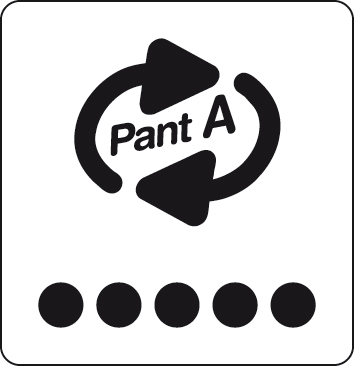
\includegraphics[width=2cm]{billeder/refund-mark.png}
\end{minipage}
  \begin{minipage}{0.8\textwidth}
    {\Large This includes glass bottles other than standard 33cl beer
    bottles (those go in the crates $\rightarrow$) bearing an official danish deposit
    mark or sticker similar to the one shown left of this text.}
\end{minipage}

\end{center}

\underskriv


\end{document}